% #############################################################################
% This is Chapter 4
% !TEX root = ../main.tex
% #############################################################################
% Change the Name of the Chapter i the following line
\fancychapter{Experimental Work \& Results}
\cleardoublepage
% The following line allows to ref this chapter
\label{chap:results}

So far, we have introduced the theme to be developed in this thesis in Chapter \ref{chap:intro}, we have presented some studies developed in this area in Chapter \ref{chap:background}, and we have presented the specific case studied approached in this thesis during Chapter \ref{chap:architecture}. In this chapter, we present the experimental procedure put into practice, and the results obtained.



\section{Initial considerations}

Before diving into the details of the experimental work, it is necessary to establish a baseline for the results obtained. Without establishing the basis it is quite difficult to know what kind of values to expect during the development of the predictive models. In order to establish a comparative basis, a baseline model was developed which can be called the Naive Model. The \textit{modus operandi} of this new model is relatively simple and is given by:

\begin{equation}
   Pred(x_{t+5}) = Pred(x_{t+10}) = Pred(x_{t+15}) = Real(x_{t}),
   \label{naive}
\end{equation}

i.e., the forecast that this model produces for each of the three cases $(t+5)$, $(t+10)$ and $(t+15)$ is exactly the value measured at instant t. The Naive Model is useful for establishing a reference point, serving as a performance comparison basis for the remaining models.

A total of 42 forecasting architectures were implemented, resulting in a total of 168 models being trained (42 architectures $\times$ 4 blocks). From the 42 implemented architectures, 3 correspond to a \ac{GRU} Vanilla implementation and 3 correspond to a \ac{LSTM} Vanilla implementation, 9 to \ac{GRU}-Encoder-Decoder and 9 to \ac{LSTM}-Encoder-Decoder, 9 to \ac{1D CNN}-\ac{GRU}-Encoder-Decoder and 9 to \ac{1D CNN}-\ac{LSTM}-Encoder-Decoder.

\section{Forecasting performance}\label{chap3:section:stage_1}

At this stage, by performing the nested cross-validation procedure detailed in section \ref{chap3:subsec:data_partition}, all the architectures were experimented in each block, firstly to optimize the hyperparameters (inner loop), and secondly, to test the models in different scenarios (outer loop). The possibility of observing the behavior of any system in different scenarios, allows the user to perform a more robust evaluation of the system in question, and adapt it based on more information. The larger the number of blocks used, the more robust the evaluation, because a larger number of different scenarios are considered. To do so, the blocks 1, 2, 3 and 4 defined before, were used. The nested cross-validation procedure implements an expanding window methodology that consists of gradually expanding the training window, which is particularly useful when there is few data available. In this case, all blocks use 2 weeks of data for validation, 2 weeks for testing, and the number of weeks of training is expanded gradually, 10 for block 1, 12 for block 2, 14 for block 3, and 16 for block 4.

The expanding nested cross-validation process described before, is put into practice with these four sets of data, where all the models are trained, validated and tested in each of the sets, and the errors presented in each of the validation and test sets are recorded. At the end of this stage, an average of the errors presented in each of the four blocks is computed and for each of the models, the combination of hyperparameters that produces the smallest error for each block, is selected as the final architecture of the model. 

The process of tuning hyperparameters is a long and time consuming process. Although the meaning of each hyperparameter and what it represents in the context of the layer is known, there is no rule dictating which hyperparamters are best for each case. It is an experimental process in which the models must be trained, and based on the validation results, the best hyperparamters should be chosen. The results obtained in the validation data are then compared for different hyperparameter combinations in each block. To speed up this process, a script \cite{code} was created, responsible for training and validating multiple combinations of hyperparameters for each of the proposed models. In total, about 84 different combinations were tested in each of the four blocks.

As explained earlier, exhaustive grid-search was implemented to test various combinations of hyperparameters for each of the models. In the layers \ac{GRU} and \ac{LSTM}, the number of units of each layer was consecutively changed.
The number of units is a positive integer that represents the dimensionality of the output space of the layer. This hyperparameter must be tuned in order to find a value for which the system performs well. However, the increase of this value represents an increase in the complexity of the model, which makes it slower. Regarding the \ac{1D CNN} layers, the hyperparameters that were tested were the number of filters - An integer that represents dimensionality of the output space (i.e. the number of output filters in the convolution), and the kernel\_size - An integer specifying the length of the 1D convolution window used. In the Max pooling layer, the pool\_size was fixed to 2 units, which means that for each pair of consecutive values, only the one with the highest value is selected, as explained in the section \ref{chap3:subsubsec:1dcnn}. In order to avoid overfitting, dropout layers with $p=0.2$ were also used.

Another hyperparameter that is common to all architectures is the dimension of the sequences introduced at the entry-level, that is, how many steps back will the model have access to perform its predictions. For this we tested several options, for example, 15 steps back (i.e. use the last 15 minutes data to predict the next 15 minutes), 60 steps back (i.e. use the last hour data to predict the next 15 minutes), and 420 steps back (i.e. use the last seven hours data to predict the next 15 minutes). Longer past time windows have also been tested, but the conclusion is that increasing this value brings more disadvantages than advantages, namely in the training time of the model. In addition, since it is intended to predict in the very short term, the influence that data collected a week ago may have on the energy behavior of the building is quite small. It is also relevant to mention that the high granularity of the data used (1 sample per minute), quickly turns the training process of any model very slow when using very large past time windows. For example, if one wants to use the data of the last week, to predict a single iteration of 15 steps, it is necessary to use 60*24*7 = 10080 steps of the past which, in practice, can quickly become quite demanding computationally. Among the three options presented, it was chosen to use the second one, where data from the last hour is used to predict the next 15 minutes. The difference in performance obtained by each of the models compared to the third option (420 steps), did not present drastic changes that would compensate the selection of the most expensive option. Compared to the past 15 steps, the use of 60 steps showed some improvements, so the second option was chosen. It is important to point out that the purpose of this choice comes from the nature of the data and the goals of the case study in question. However, it may be developed in future work the use not only of more values from the past for the production of each iteration, but also the modification of the granularity of the data used.

In Table \ref{valres}, the reader may consult the results of the nested cross-validation process, which consists of an average of the errors presented in blocks 1, 2, 3 and 4. Table \ref{valres} is divided into two major parts. In the first part, the \ac{RMSE}, \ac{MSE} and \ac{MAE} validation values are presented for each one of the models, which refers to the forecast of the available power in 5, 10 and 15 minutes. All these values are an average of the results obtained for each of the four blocks, as defined in section \ref{chap3:subsec:data_partition}. It should be noted that, the two Vanilla models produce only 3 values, due to the nature of "many-to-one" models. On the other hand, the remaining models, "many-to-many", produce whole sequences with 15 values. For the first two models, the errors shown in Table \ref{valres} result from direct comparison between the first value produced by the model and the actual power available in 5 minutes, a process that is equally valid for the other two measures. For the Encoder-Decoder models, the errors were calculated by comparing the fifth value of the sequence generated by the model, with the fifth value of the measured sequence for the same time-interval, and so on for the remaining two readings. At the end, the Total Validation section corresponds to the average value of each metric for the three measures. It was decided to compute this value to enable the global evaluation of each of the models, and not just the individual evaluation for each one of the time targets. With these average metrics, it is then possible to compare the performance of models at a global scale. The second part of Table \ref{valres} is similar to the first part described before, with the difference of detailing data related to the test sets instead.

% Table generated by Excel2LaTeX from sheet 'Tabel Creation'
\begin{table}[htbp]
  \centering
  \caption{Selected models resulting from window cross-validation procedure.}
    \begin{tabular}{r|c|cc|cccc}
    \multicolumn{1}{c|}{\multirow{2}[1]{*}{\textbf{Model}}} & \multirow{2}[1]{*}{\textbf{Naïve}} & \multicolumn{2}{c|}{\textbf{Vanilla}} & \multicolumn{4}{c}{\textbf{Encoder-Decoder}} \\
      &   & GRU & LSTM & GRU-GRU & LSTM-LSTM & CNN-GRU & CNN-LSTM \\
    \midrule
    \textbf{Val. (t+5)} &   &   &   &   &   &   &  \\
    RMSE (E-02) & 2.674 & 2.484 & 2.626 & 2.572 & 2.605 & 2.910 & 2.876 \\
    MSE(E-03) & 0.716 & 0.618 & 0.691 & 0.664 & 0.681 & 0.850 & 0.829 \\
    MAE (E-02) & 1.891 & 1.787 & 1.913 & 1.893 & 1.947 & 2.187 & 2.175 \\
    \textbf{Val. (t+10)} &   &   &   &   &   &   &  \\
    RMSE (E-02) & 3.118 & 2.912 & 3.020 & 2.978 & 3.007 & 3.212 & 3.213 \\
    MSE(E-03) & 0.973 & 0.848 & 0.913 & 0.889 & 0.906 & 1.034 & 1.033 \\
    MAE (E-02) & 2.247 & 2.115 & 2.213 & 2.191 & 2.236 & 2.405 & 2.422 \\
    \textbf{Val. (t+15)} &   &   &   &   &   &   &  \\
    RMSE (E-02) & 3.458 & 3.204 & 3.365 & 3.257 & 3.338 & 3.509 & 3.539 \\
    MSE(E-03) & 1.197 & 1.027 & 1.133 & 1.062 & 1.116 & 1.234 & 1.253 \\
    MAE (E-02) & 2.517 & 2.333 & 2.473 & 2.389 & 2.488 & 2.628 & 2.666 \\
    \midrule
    \textbf{Total Val.} &   &   &   &   &   &   &  \\
    RMSE (E-02) & 3.083 & 2.867 & 3.004 & 2.935 & 2.984 & 3.210 & 3.209 \\
    MSE(E-03) & 0.962 & 0.831 & 0.912 & 0.872 & 0.901 & 1.039 & 1.038 \\
    MAE (E-02) & 2.219 & 2.079 & 2.200 & 2.158 & 2.224 & 2.407 & 2.421 \\
    \midrule
    \textbf{Test (t+5)} &   &   &   &   &   &   &  \\
    RMSE (E-02) & 2.713 & 2.509 & 2.694 & 3.047 & 3.036 & 3.370 & 3.217 \\
    MSE(E-03) & 0.737 & 0.630 & 0.726 & 0.977 & 0.945 & 1.152 & 1.049 \\
    MAE (E-02) & 1.903 & 1.785 & 1.934 & 2.263 & 2.267 & 2.508 & 2.414 \\
    \textbf{Test (t+10)} &   &   &   &   &   &   &  \\
    RMSE (E-02) & 3.149 & 2.955 & 3.103 & 3.425 & 3.489 & 3.693 & 3.537 \\
    MSE(E-03) & 0.993 & 0.874 & 0.963 & 1.211 & 1.247 & 1.380 & 1.261 \\
    MAE (E-02) & 2.238 & 2.115 & 2.246 & 2.534 & 2.593 & 2.746 & 2.644 \\
    \textbf{Test (t+15)} &   &   &   &   &   &   &  \\
    RMSE (E-02) & 3.492 & 3.236 & 3.448 & 3.671 & 3.823 & 3.956 & 3.839 \\
    MSE(E-03) & 1.220 & 1.048 & 1.189 & 1.380 & 1.490 & 1.580 & 1.482 \\
    MAE (E-02) & 2.500 & 2.310 & 2.491 & 2.699 & 2.844 & 2.944 & 2.862 \\
    \midrule
    \textbf{Total Test} &   &   &   &   &   &   &  \\
    RMSE (E-02) & 3.118 & 2.900 & 3.082 & 3.381 & 3.449 & 3.673 & 3.531 \\
    MSE(E-03) & 0.983 & 0.850 & 0.959 & 1.189 & 1.228 & 1.371 & 1.264 \\
    MAE (E-02) & 2.214 & 2.070 & 2.224 & 2.499 & 2.568 & 2.733 & 2.640 \\
    \end{tabular}%
  \label{valres}%
\end{table}%


Before proceeding to the analysis of the results obtained, it is important to clarify that, from the user point of view, the best architecture will be the one that minimizes the validation \ac{MSE}. This metric is chosen because the validation data is the only data that the user has access before the implementation of the developed system.

Let's first compare the performance between the Vanilla \ac{GRU} model with the Vanilla \ac{LSTM} model. As explained in section \ref{chap3:subsec:artificial_neural_networks}, these two architectures were introduced in order to avoid the exploding and vanishing gradient problems in \ac{RNN}s. However, they are different architectures, with different characteristics. Given their simpler architecture, the \ac{GRU}s typically train faster and require less training data. On the other hand, the \ac{LSTM}s, given their complexity, have more ability to remember large sequences than the \ac{GRU}s, managing to establish dependencies with a larger time frame. All tested architectures use \ac{GRU} layers or \ac{LSTM} layers. The goal is to develop a comparative analysis between these two types of \ac{RNN}s.

As for the validation data, one can start the analysis by Vanilla models. It is possible to verify that for the three proposed situations ((t+5), (t+10) and (t+15)), the \ac{GRU} architecture surpassed the \ac{LSTM} architecture. According to the total validation \ac{MSE} of these two models, it can indeed be verified that the \ac{GRU} model is the model of choice with respect to the Vanilla architectures. This can be justified by the fact that the problem has been formulated to predict data for the next 15 minutes based on data from the last 60 minutes. At the problem scale, the previous 60 minutes are a relatively small size, small enough that the capabilities of the \ac{LSTM} model do not stand out from the results obtained by the \ac{GRU} model. If the user wants to opt for a simpler model, he/she should then choose the \ac{GRU} Vanilla model. For Encoder-Decoder architectures, in the case of the \ac{GRU}-\ac{GRU} and \ac{LSTM}-\ac{LSTM} models, it can be seen that the \ac{GRU} superiority over \ac{LSTM} is preserved, since the total \ac{MSE} for the first model is slightly lower than the value presented for the second model. If one inspects each of the three measurements, it can also be verified that in all of them the \ac{GRU} model is superior to the \ac{LSTM} model. If the user wants to choose an Encoder-Decoder model, then he/she must choose the \ac{GRU}-\ac{GRU}  model since during the whole validation process it was the model whose performance was superior. Regarding Hybrid Encoder-Decoder architectures, \acs{CNN}-\ac{GRU} and \acs{CNN}-\ac{LSTM}, it can be verified that, unlike the other architectures, the \ac{GRU} model does not present a better performance than the \ac{LSTM} model. For instant (t+5), the GRU model has a worse performance than the \ac{LSTM} model, for the instant (t+10) the errors obtained by the two models are almost the same, and for the instant (t+15) the \ac{GRU} model exceeds the \ac{LSTM} model for the first time. It then becomes difficult to define which of the two models has the best performance for the case where the encoder is composed of a \ac{1D CNN} layer. This can also be confirmed by the analysis of the total validation \ac{MSE} value produced by both models, which is practically the same. Since the \ac{GRU} layers present a simpler architecture and a lower running time, the user should choose to implement the Hybrid \ac{CNN}-\ac{GRU} model. Overall, one must then choose from all architectures, those that employ \ac{GRU} layers over the ones of that employ \ac{LSTM}.

When comparing the validation results of all architectures with the results obtained by the Naive model, one quickly realizes that the Hybrid \ac{CNN}-\ac{GRU} and \ac{CNN}-\ac{LSTM} models do not perform well, since the errors obtained in the validation data are higher than the base values established by the Naive model. This may be due to several reasons, among which is the use of maxpooling after the \ac{1D CNN} layers. Although the maxpooling operation is important in reducing the dimensionality of the problem (which implies a drastic reduction in model run time), it has the disadvantage of reducing the granularity of the samples passed to the encoder vector. In this specific case, maxpooling of two units was used, which means that only half of the sequences coming from the convolutional layers are considered. This condition reduces by half the running time of the models, but there is a price to pay, which manifests itself in the increase of the error obtained, as verified by F. Chollet in \cite{cnn1}. Another reason that might be related with these performance results in the validation data is the fact that, for the case under study, the use of a \ac{CNN} layer as encoder is simply a worse option than using a \ac{RNN} layer. The choice of \ac{CNN} layers for encoding was based on the premise that \ac{CNN} layers are typically good for extracting the importance of features in a set of several features. However, for the case under study, it was verified that the use of this type of encoder did not yield better results. It is curious to see that the simplest model, \ac{GRU} Vanilla, is the one that presents the lowest \ac{MSE} value, followed by the \ac{GRU}-\ac{GRU} Encoder-Decoder model. \ac{GRU} layers clearly outperformed \ac{LSTM} layers in the validation data, showing to be the best option for the problem under study. One would expect a user to choose to implement the \ac{GRU} Vanilla model. If the user decided to use an Encoder-Decoder model, it would be advisable to opt for the \ac{GRU}-\ac{GRU}, as it performed better than the \ac{LSTM} Encoder-Decoder, and both Hybrid Encoder-Decoder models. 

Moving on to the test phase, where the models were tested on a data set never seen before, despite having implemented multiple techniques to prevent it, there are signs of overfitting as the \ac{GRU}-Encoder-Decoder  and \ac{LSTM}-Encoder-Decoder models are no longer superior to the Naive model. In fact, the Vanilla models were the only ones that maintained the behavior presented in the validation phase, and that outperformed the Naive model. The results obtained make us question the applicability of Encoder-Decoder architectures to the specific case, since the complexity that comes from implementing this sort of architectures has not offered any advantage over simpler architectures. One can also verify that the increase in the complexity of the models presents an inverse relationship with the performance obtained, which may lead us to conclude that, given the specificities of the case under study, the implementation of Encoder-Decoder architectures is in no way advantageous in predicting the available power of the building in a short period of time. Furthermore, the applicability of architectures to this specific case may also be questioned. As can be seen from the test data, the \ac{GRU} Vanilla model showed an improvement of 6.9\% over the \ac{RMSE} value obtained by the Naive model, and the \ac{LSTM} Vanilla model an improvement of 1.15\%. 


%TEORICO 1 OU DUAS REFERÊNCIAS
 
In the practical case of the EDP building, it must be understood that currently the building does not have any power available forecast system implemented. Even the implementation of the \ac{CNN}-\ac{GRU} Encoder-Decoder model (the one with the worst performance in the test data), would bring numerous advantages in what is the activity of the \ac{EVCS} since currently this system does not use any future values in the optimization of the charging of \ac{EV}s. On the other hand, it would be inefficient to implement a \ac{ML}  system whose performance is inferior to the Naive Model. In practice, the operating mode of the Naive Model is to assume that the available power in the building in the next 15 minutes is equal to the available power at the current time. The implementation of a \ac{ML} system that runs in real time has some costs, namely the hosting of the code, the hardware capable of running the developed system, and the whole energy cost. This way, one should only consider to implement a system whose performance is superior to the performance of the Naive model, since the associated costs have to be compensated by a significant performance improvement. Fortunately, both the \ac{GRU} Vanilla model and the \ac{LSTM} Vanilla model have outperformed the Naive model, so for this case study, it can be said that it is worth implementing a forecasting system based on \ac{ML} methodologies.

\section{Confidence intervals}\label{chap3:section:stage_3}

The purpose of this work is to predict a value for the available power for the next 5, 10 and 15 minutes, but it would be interesting to set a minimum and a maximum value for each of these three forecasts. In other words, it would be important to be able to project the confidence intervals of the forecasts carried out. 

In order to project the confidence interval of a forecast from a set of points $x(t, ..., N)$, multiple sets of values are needed for the same interval, that is to say that based on the same input data, the model would have to be able to generate several forecasts for the same instant, but this does not happen for standard architectures. As it is known, after the training stage in which the weights are defined, \ac{ANNs} become deterministic functions, which means that for the same input, the same predicted output will always be produced, regardless of the number of times the algorithm runs. One is then faced with a limitation, the impossibility of obtaining several values for the same instant, so that a confidence interval of the forecast can be computed.

In 2017, Zhu et al. \cite{uber} proposed a technique to tackle this problem. The principle consists in adapting the predictive model so that it can return multiple (different) predictions by applying dropout in the forecasting process. As discussed in section \ref{chap3:subsubsec:regularization_techniques}, one of the most common techniques to avoid overfitting is to use dropout layers. Usually, these layers are active in the training process, in order to introduce some error in the model to prevent it from overadapting to the data provided. The application of dropout "turns off" a randomly chosen fraction of the units of the model. But in the testing phase, these layers are disabled. Applying dropout in the testing process would imply that the model ceases to be deterministic, that is, for the same input, different outputs are generated each time forecasts are made. 
This principle is also known as \acf{MCD} \cite{uber2}, which dictates that the uncertainty of the model can be estimated by sample variance of the forecasts of the adapted model in some repetitions. For example, if for each input sequence, 100 distinct output sequences are predicted, assuming the dropout is maintained, all 100 sequences are different. By averaging the 100 sequences, one obtains an average forecast of the model, which can be assumed to be the actual result of the model forecast, that can be called \ac{MCD} Forecast. On the other hand, since for each instant one has 100 different sequences, the standard deviation of the 100 sequences can then be used to calculate the confidence interval of each of the values and, ultimately, the complete sequence. Assuming that the forecasts have a normal distribution $N(\mu, \sigma^2)$, with a mean $\mu$ and a standard deviation $\sigma$, it is then possible to determine the confidence intervals given by: 

\begin{equation}
    [\hat{y}^* - z_{\frac{\alpha}{2}}\mu,\ \hat{y}^* + z_{\frac{\alpha}{2}}\mu], 
\end{equation}

where $\hat{y}^* = \frac{1}{B}\sum_{b=1}^B\hat{y_b}$, and $\mu = \sqrt{\frac{1}{B}\sum_{b=1}^B(\hat{y_b} -\hat{y}^*)^2}$. In order to to compute the 95\% confidence interval, for example, the parameters should be $\alpha=0.05$ and $z_{\frac{\alpha}{2}}= 1.92$ . 

Another consideration that should be made is the selection of the parameter $p$ (value between o and 1 that indicates the percentage of values that are dropped out) in the \ac{MCD}. If the $p$ is too large, the forecasts generated will be quite sparse, which in turn implies that the confidence intervals created will be too large. On the other hand, if the $p$ is too small, the forecasts made will be too similar to each other, which results in very small confidence intervals. When $p$ value is ideal, there is an almost perfect correspondence between the confidence interval and the values obtained. For the problem in question, the parameter $p$ of the \ac{MCD} was tested for various values, and it was concluded that a good value would again be $p = 0.2$. 

In the standard models, which apply dropout only in the training process, only one forecast sequence is produced, which can be called Standard Dropout Forecast. In the case where dropout is applied both in training and test sets, a set of $N$ sequences, defined by the user, is obtained. The forecast produced in this second case is an average of the $N$ sequences produced, which can be called \ac{MCD}.

Again, the nested cross-validation process was implemented where the 4 blocks were used to train, validate and test the models. In order to compare the results obtained with and without the application of \ac{MCD}, Table \ref{tab:mctab} shows the test \ac{RMSE} values for the six models, with and without the application of \ac{MCD}.

\begin{table}[htbp]
  \centering
  \caption{Standard Dropout vs Monte Carlo Dropout results.}
    \begin{tabular}{r|c|cc|cccc}
    \multicolumn{1}{c|}{\multirow{2}[1]{*}{\textbf{Model}}} & \multirow{2}[1]{*}{\textbf{Naïve}} & \multicolumn{2}{c|}{\textbf{Vanilla}} & \multicolumn{4}{c}{\textbf{Encoder-Decoder}} \\
      &   & GRU & LSTM & GRU-GRU & LSTM-LSTM & CNN-GRU & CNN-LSTM \\
    \midrule
    \textbf{Test (t+5)} &   &   &   &   &   &   &  \\
    RMSE (E-02) & \multirow{2}[0]{*}{2.713} & 2.509 & 2.694 & 3.047 & 3.036 & 3.370 & 3.217 \\
    RMSE MC (E-02) &   & 2.588 & 2.746 & 3.291 & 3.464 & 4.225 & 3.980 \\
    \textbf{Test (t+10)} &   &   &   &   &   &   &  \\
    RMSE (E-02) & \multirow{2}[0]{*}{3.149} & 2.955 & 3.103 & 3.425 & 3.489 & 3.693 & 3.537 \\
    RMSE MC (E-02) &   & 3.069 & 3.213 & 3.661 & 3.822 & 4.484 & 4.319 \\
    \textbf{Test (t+15)} &   &   &   &   &   &   &  \\
    RMSE (E-02) & \multirow{2}[1]{*}{3.492} & 3.236 & 3.448 & 3.671 & 3.823 & 3.956 & 3.839 \\
    RMSE MC(E-02) &   & 3.377 & 3.894 & 3.894 & 4.087 & 4.720 & 4.581 \\
    \midrule
    \textbf{Total Test} &   &   &   &   &   &   &  \\
    RMSE (E-02) & \multirow{2}[0]{*}{3.118} & 2.900 & 3.082 & 3.381 & 3.449 & 3.673 & 3.531 \\
    RMSE MC (E-02) &   & 3.011 & 3.284 & 3.616 & 3.791 & 4.476 & 4.293 \\
    \end{tabular}%
  \label{tab:mctab}%
\end{table}%

Looking at the data in Table \ref{tab:mctab}, one can see that while the addition of \ac{MCD} can bring the advantage of allowing the stipulation of confidence intervals of the forecasts performed, in none of the models the performance obtained has improved compared to the standard version of the models. Furthermore, the \ac{LSTM} Vanilla model is no longer superior to the Naive model with the application of \ac{MCD}. The only model that continues to present an acceptable behaviour is once again the \ac{GRU} Vanilla, which although it has shown a 3.83\% increase in \ac{RMSE} over its standard version, continues to outperform the Naive model. It can also be seen that with the increased complexity of the model, there is also an increase in the discrepancy between the value of \ac{RMSE} and \ac{RMSE} MC, which may indicate that even after the tests performed, the value of $p$=0.2 used in the \ac{MCD} may not be ideal for all models. In Figure \ref{mtcdrop} one can see the results of applying the \ac{MCD} method for all the six models developed.

\begin{figure}[h!]
\captionsetup[subfigure]{position=b}
\centering
\subcaptionbox{GRU Vanilla\label{mc1}}{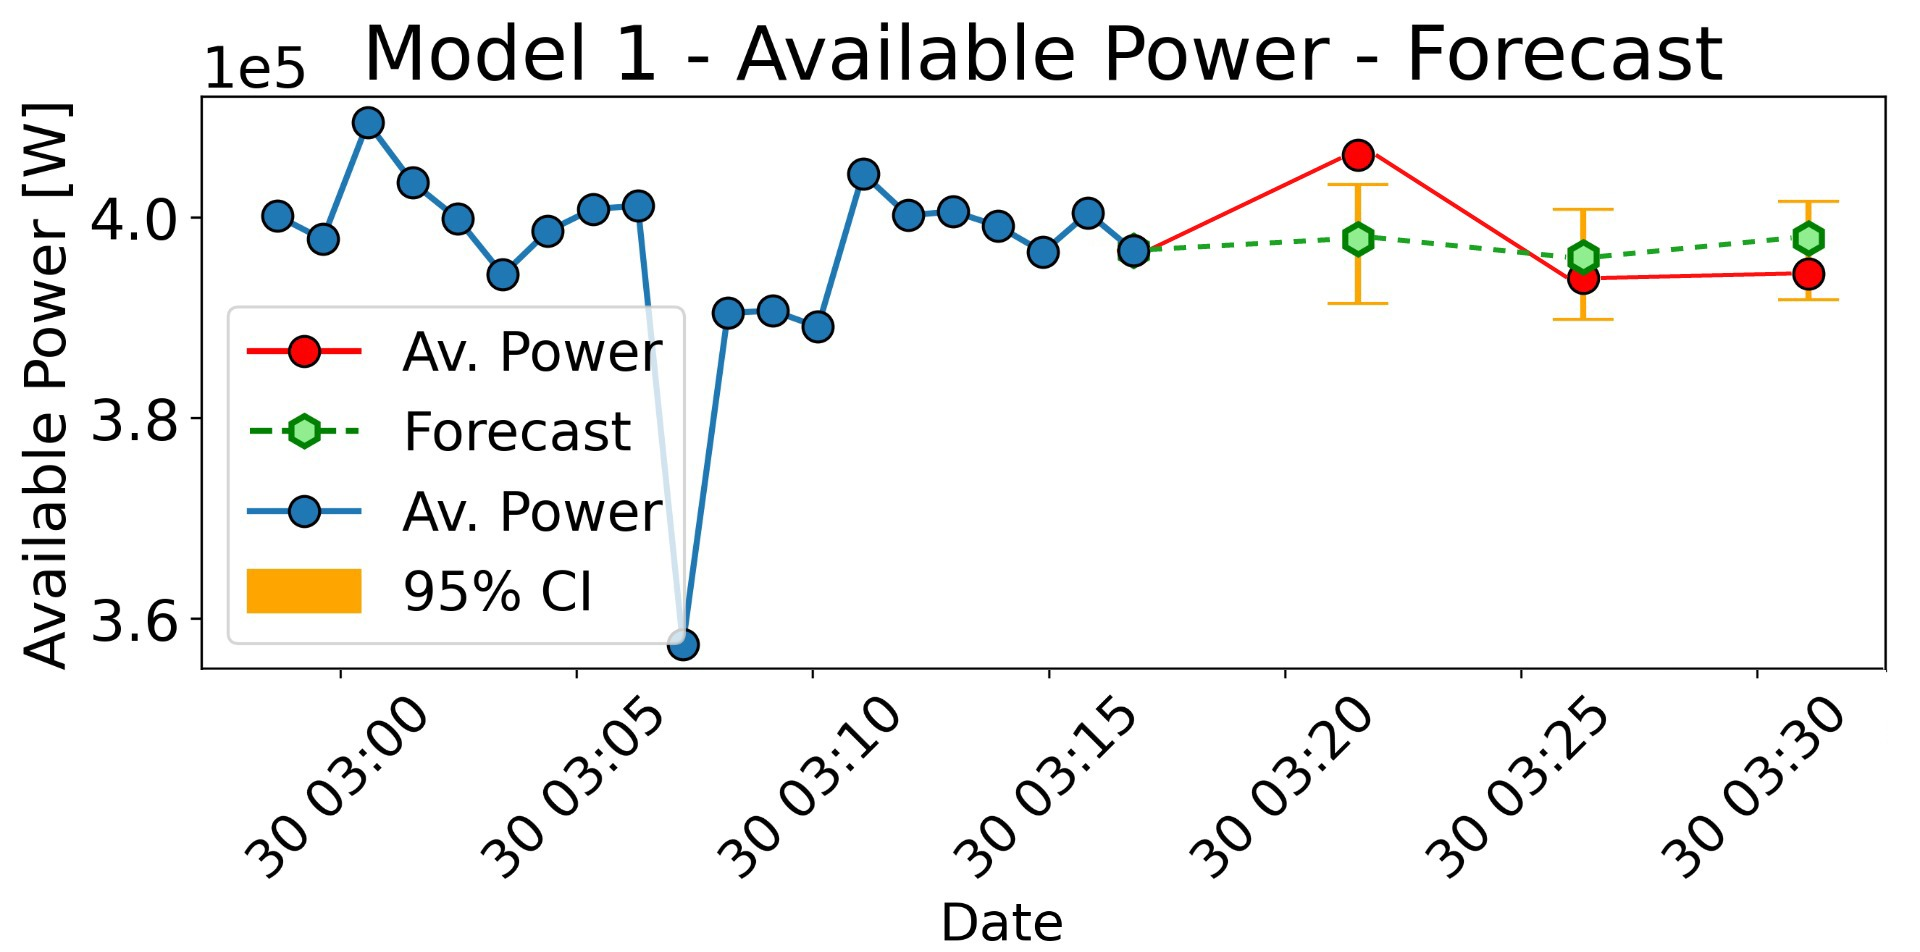
\includegraphics[width=.49\linewidth]{Images/7.jpeg}}
\subcaptionbox{LSTM Vanilla\label{mc2}}{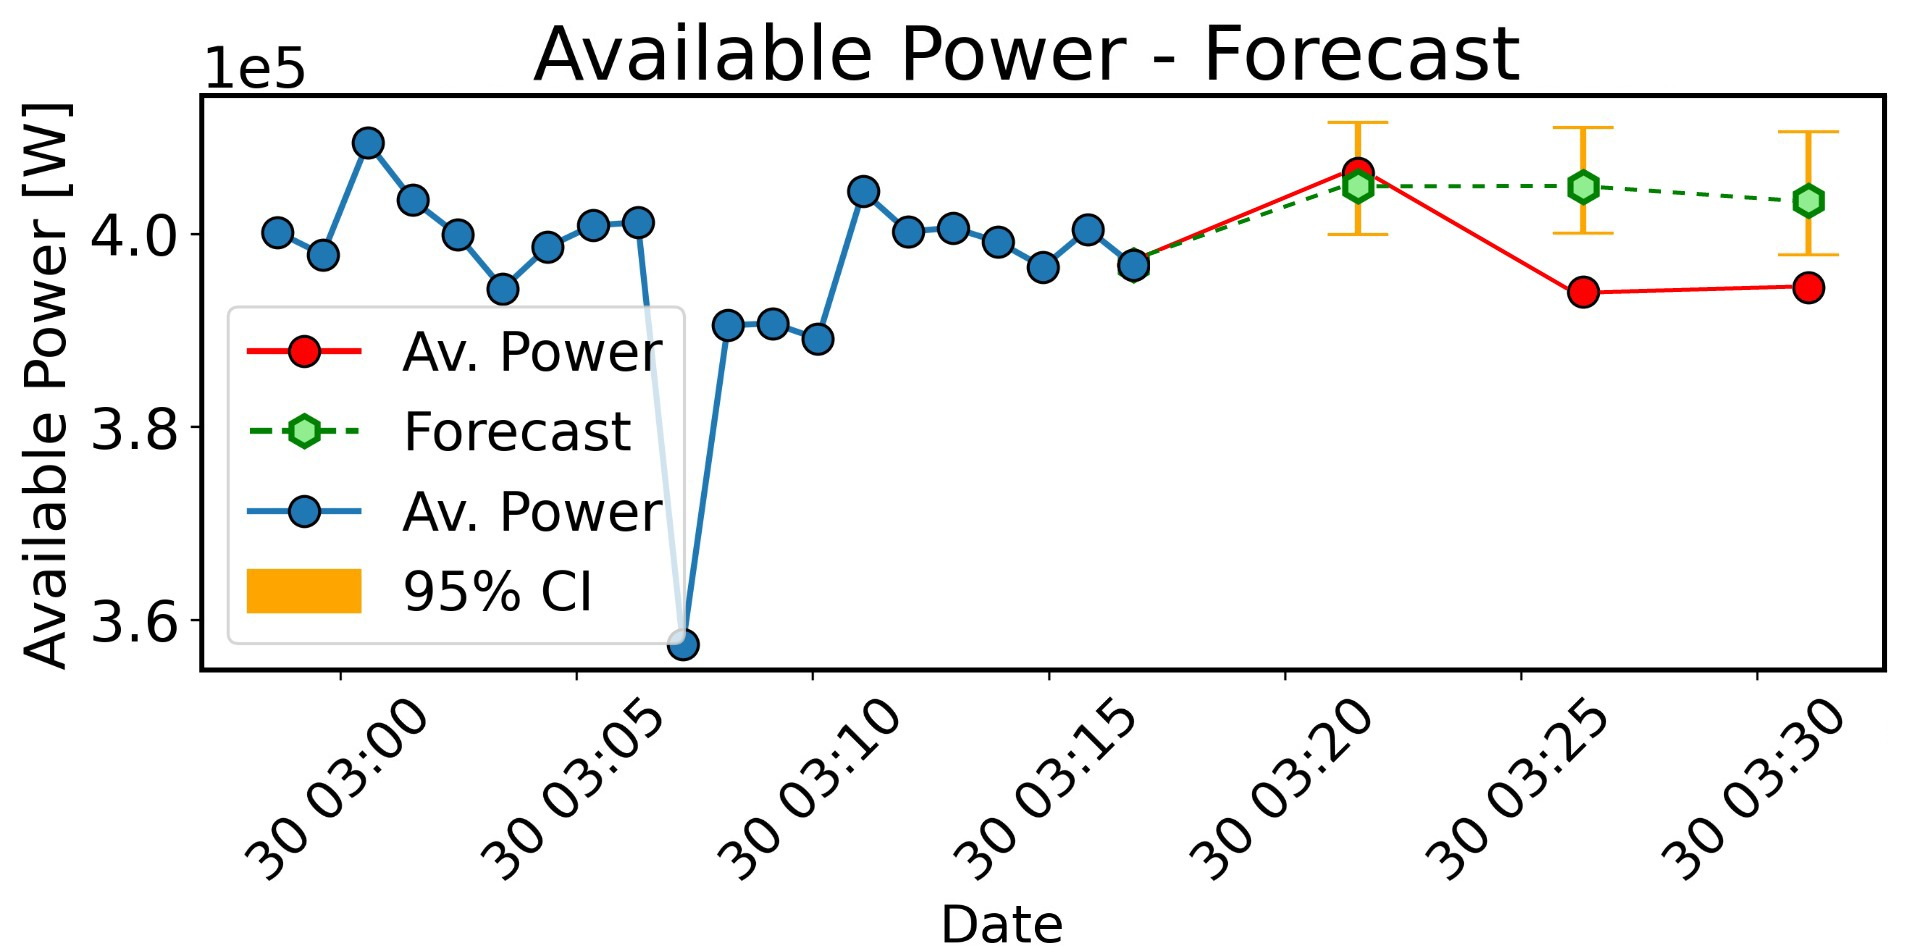
\includegraphics[width=.49\linewidth]{Images/8.jpeg}}
\subcaptionbox{GRU Encoder-Decoder\label{mc3}}{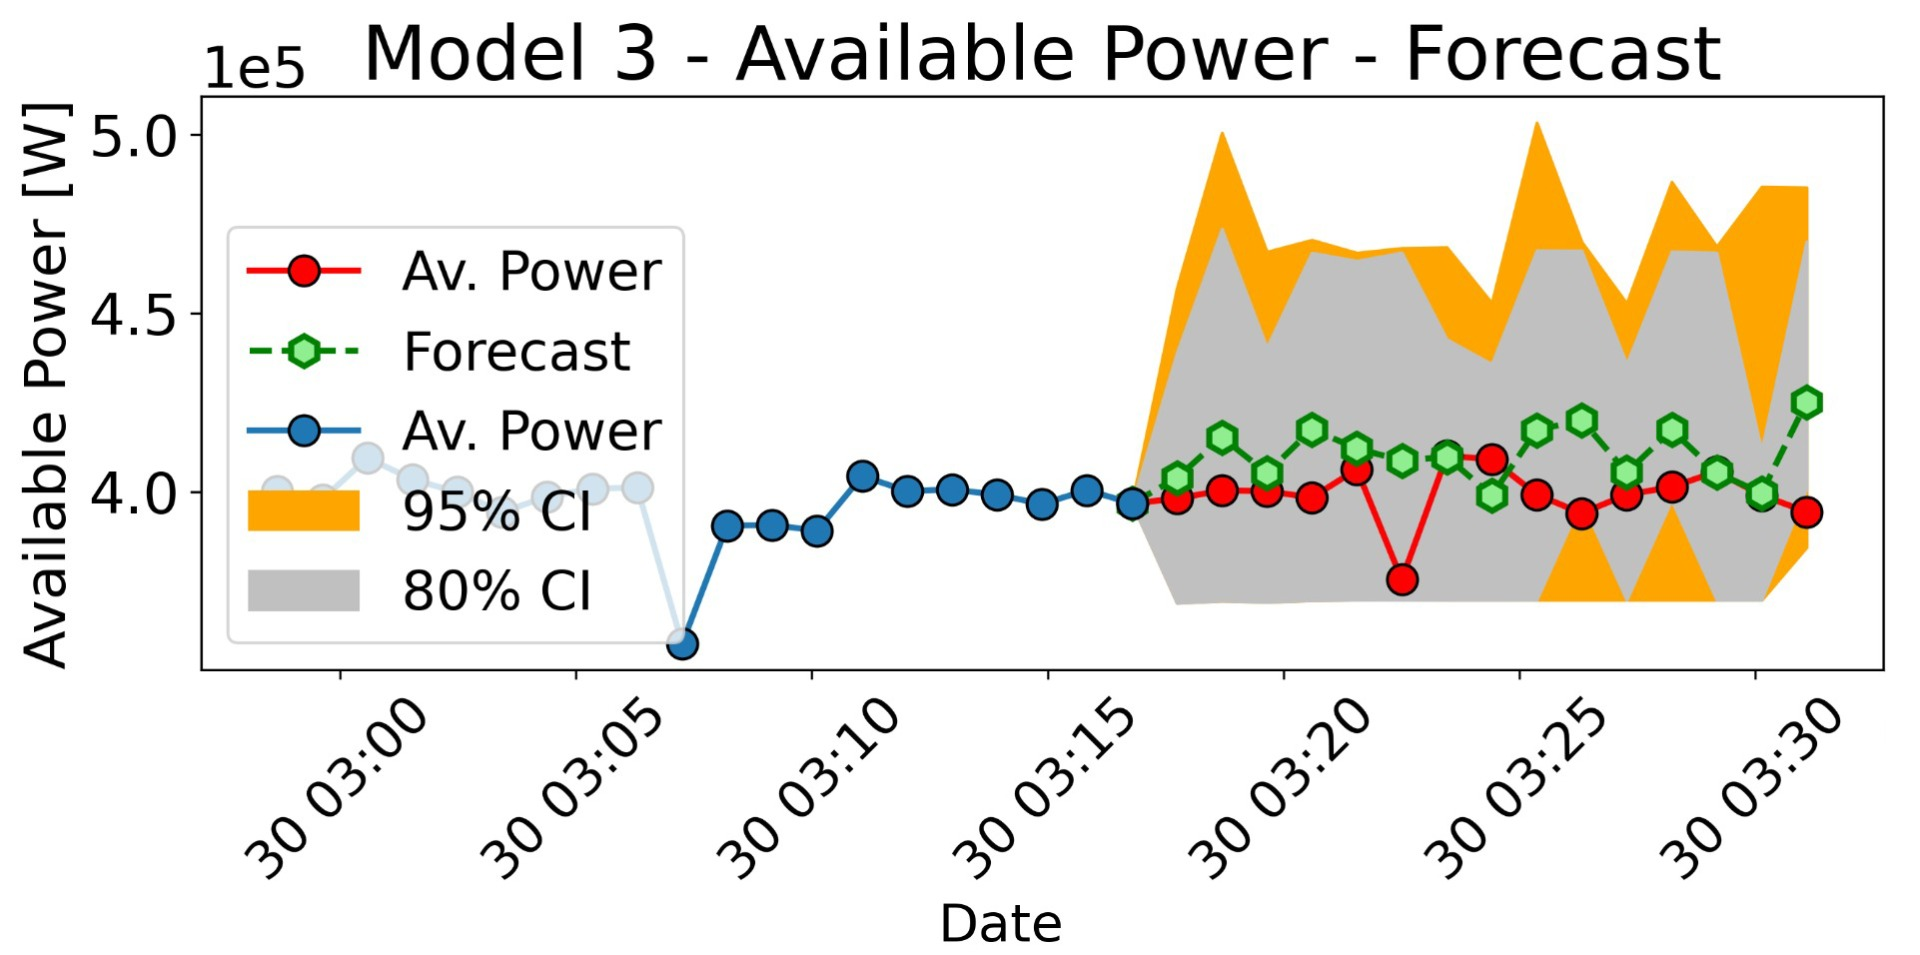
\includegraphics[width=.49\linewidth]{Images/9.jpeg}}
\subcaptionbox{LSTM Encoder-Decoder\label{mc4}}{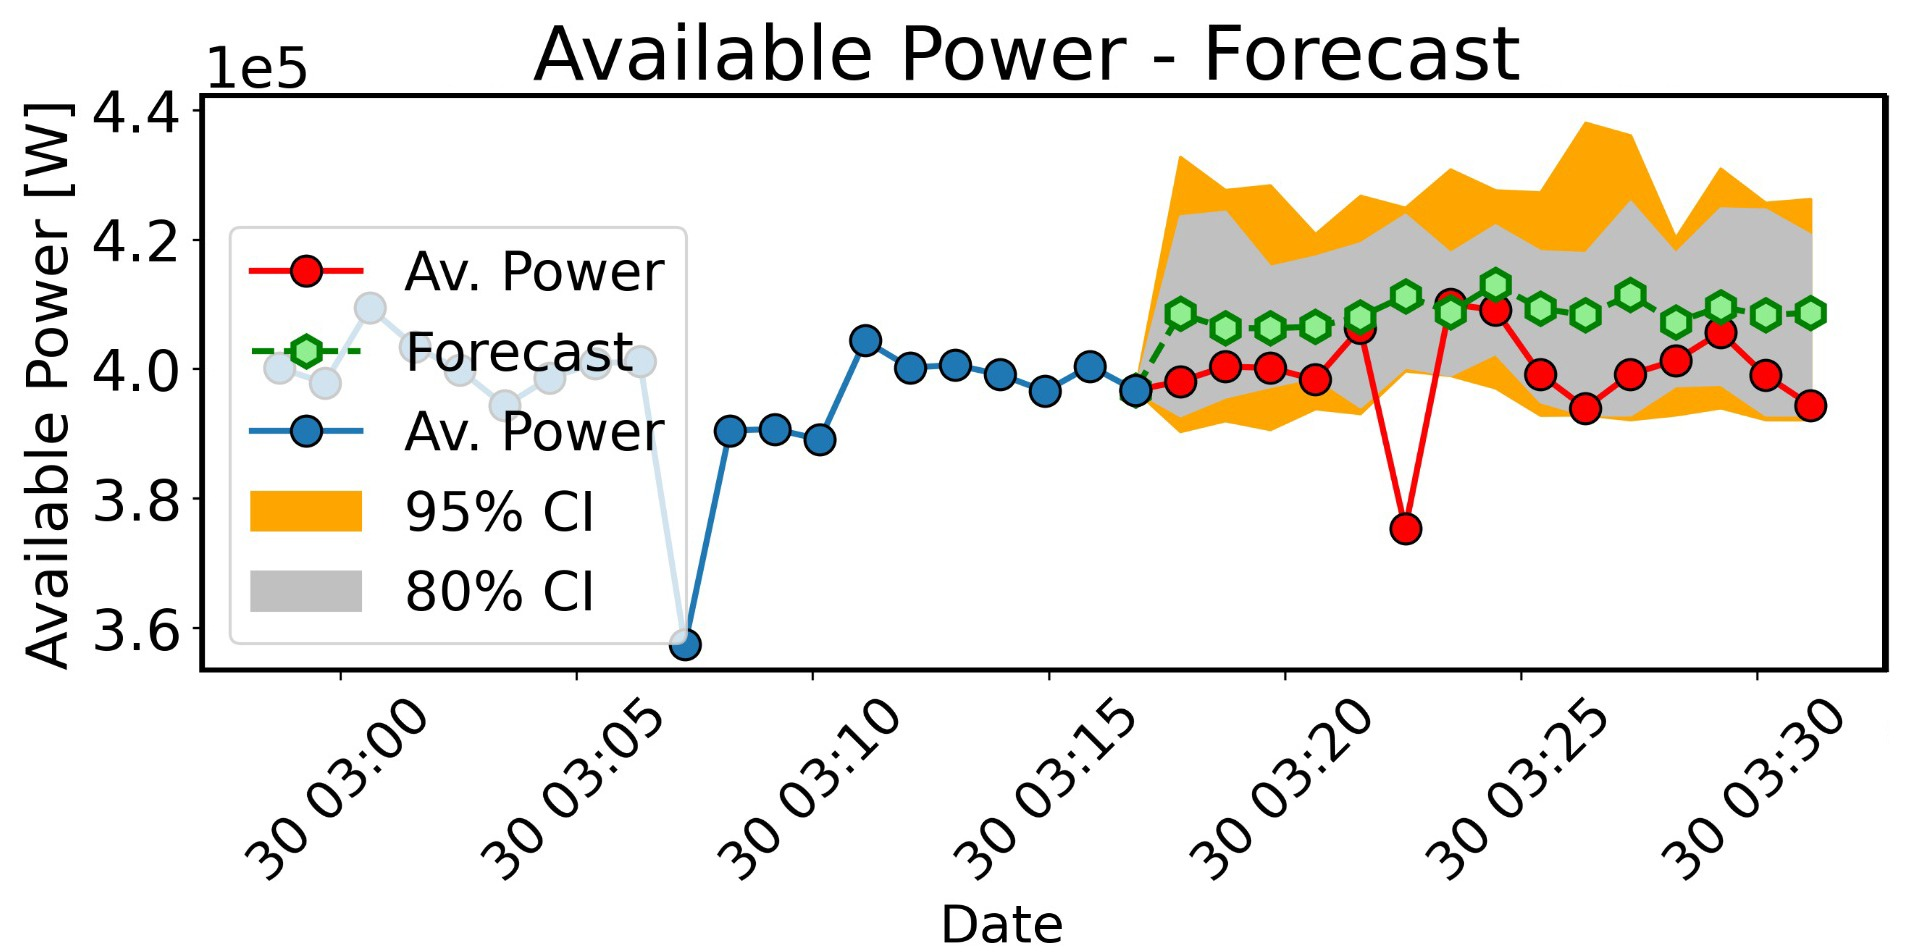
\includegraphics[width=.49\linewidth]{Images/10.jpeg}}
\subcaptionbox{CNN-GRU Encoder-Decoder\label{mc5}}{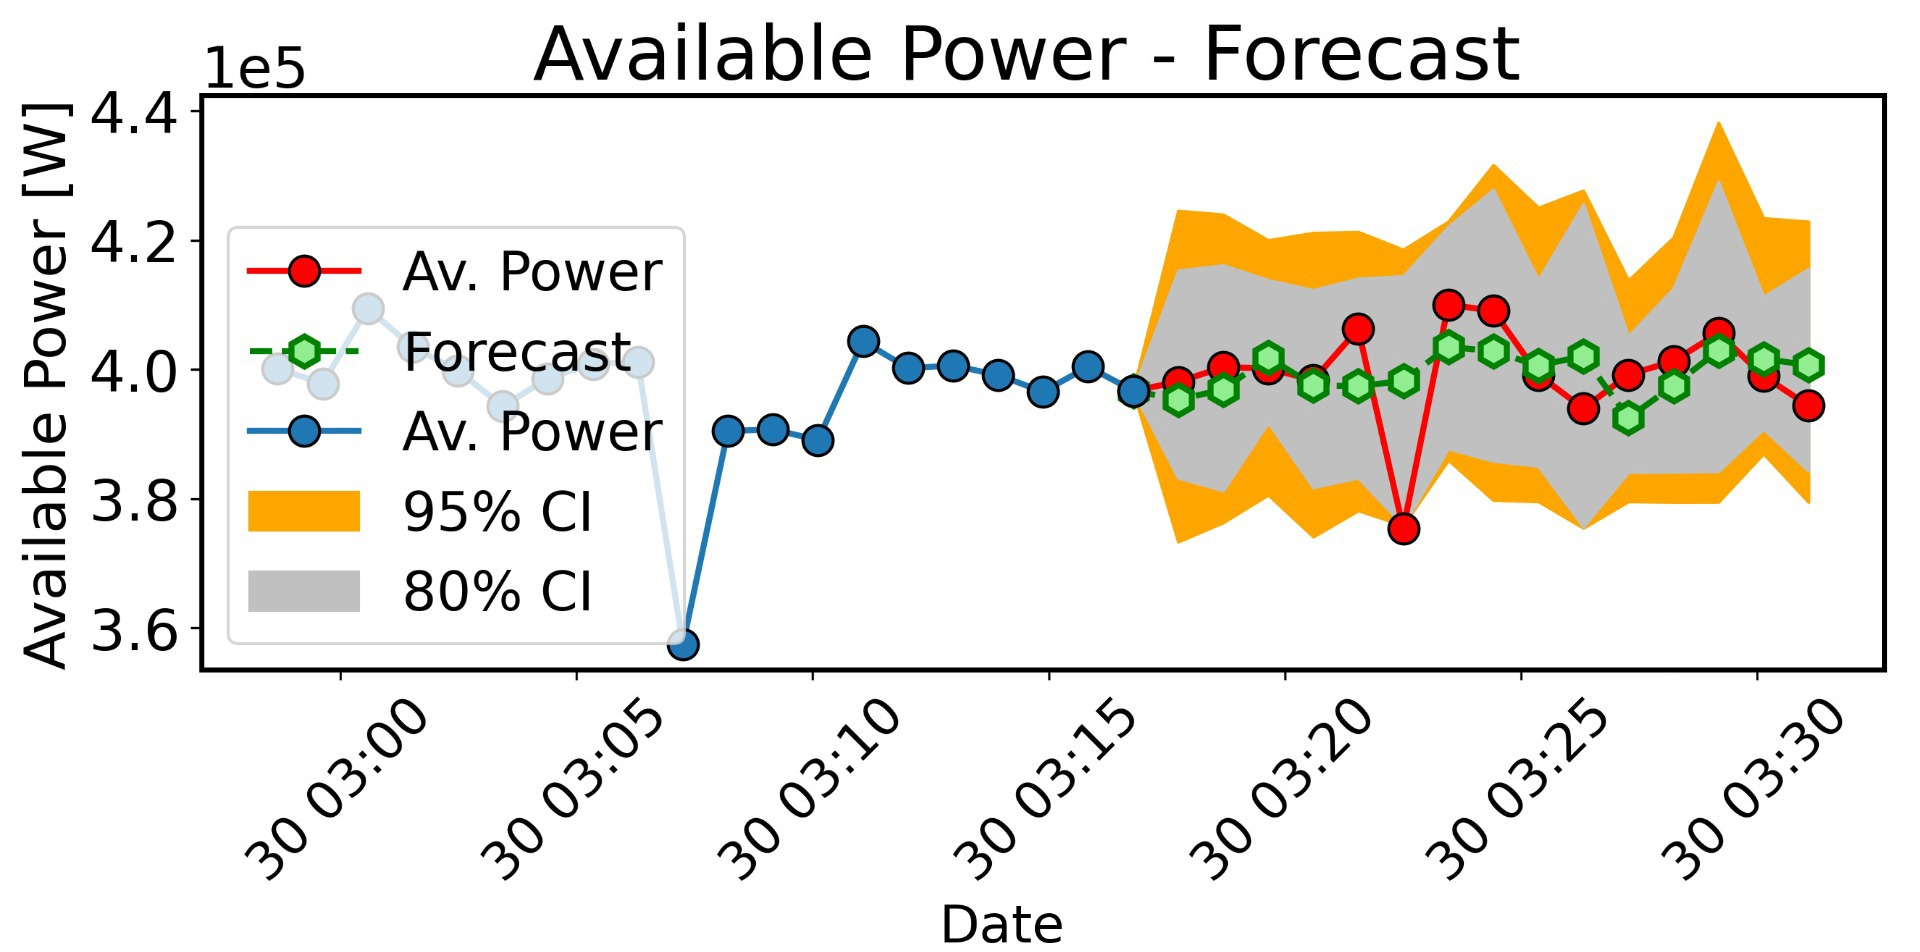
\includegraphics[width=.49\linewidth]{Images/11.jpeg}}
\subcaptionbox{CNN-LSTM Encoder-Decoder\label{mc6}}{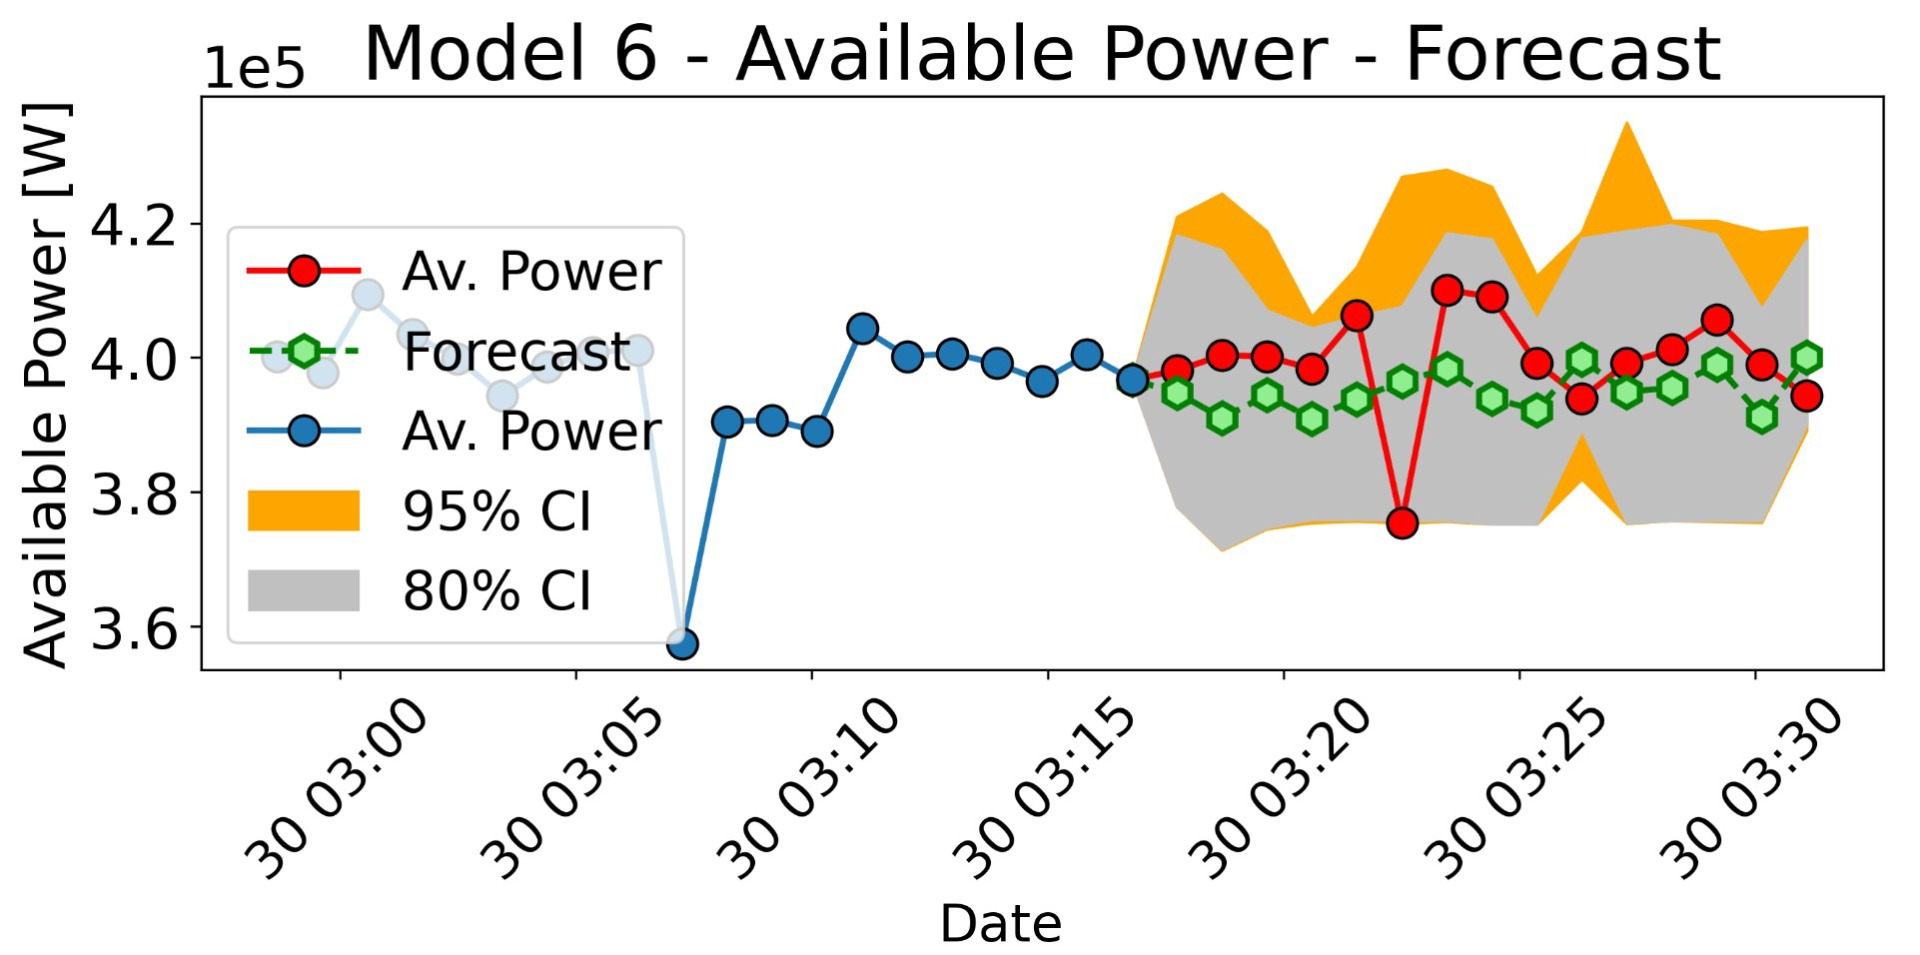
\includegraphics[width=.49\linewidth]{Images/12.jpeg}}

\caption{Available power forecast and respective confidence intervals.}
\label{mtcdrop}
\end{figure}


Looking at Figure \ref{mtcdrop}, one should mention that the charts present the same scenario for the 6 models, a forecast performed on May 30, 2020 around 3pm. The real values of the available power in the building are represented in blue for the past and in red for the values that are to be predicted. The green values represent the average $N$ forecasts performed, and are considered to be the predicted sequence. For visualization purposes, for the first two models only the 95\% confidence interval is represented in orange, since these two models produce only one vector with the forecasts for each of the three points. For the remaining four models, besides the 95\% confidence interval, the 80\% confidence interval is also represented in grey, and the respective area filled by the confidence intervals, since these models are responsible for predicting the entire sequence and not just the 3 data points. These graphs are purely illustrative and detailed analyses should not be carried out based on this information, but it is possible to verify that when \ac{MCD} is introduced, the Encoder-Decoder models are much more susceptible to oscillation, which is according to the data in Table \ref{tab:mctab}. These graphical representations are also useful to provide to the reader an idea of the final interface that will be made available to the user. 

It should be remembered that the forecasts resulting from the application of Standard Dropout are generated with a single iteration of the forecast process, while the models that apply MC Dropout result from $N$ iterations. The more iterations carried out, the more accurate the stipulated interval will be, however the forecasting process will also take longer. It is then necessary to balance the value of $N$ with the time that $N$ iterations take to be processed. In very short-term forecasting models, as is the case, this factor is preponderant since the granularity of the data is very high and the forecasts should be immediate. It is also a factor that is directly linked to the available computing capacity.


Overall, the decision of whether or not to use MCD is up to the user. If a forecast with the least possible error is desired, the user should choose to use the standard version of the model. If the user wants to give up some performance in order to have access to the confidence intervals, he/she can opt for the MCD version of the model. 

In the specific case of \ac{EDP}, the second option is particularly interesting because, through the computation of the confidence intervals, the user has access to several forecasts, among them, one that can be consider the best possible case (where the available power is higher), and one that can consider the worst possible case (where the available power is lower). These two scenarios correspond to the limits observed in the confidence intervals of Figure \ref{mtcdrop}. Access to the optimistic case and the pessimistic case are one of the achievements of this thesis, as it provides the user and ultimately the \ac{EVCS} more information to support his process of \ac{EV} charging optimization.
